\begin{figure}[htb]
    \hspace{12mm}
    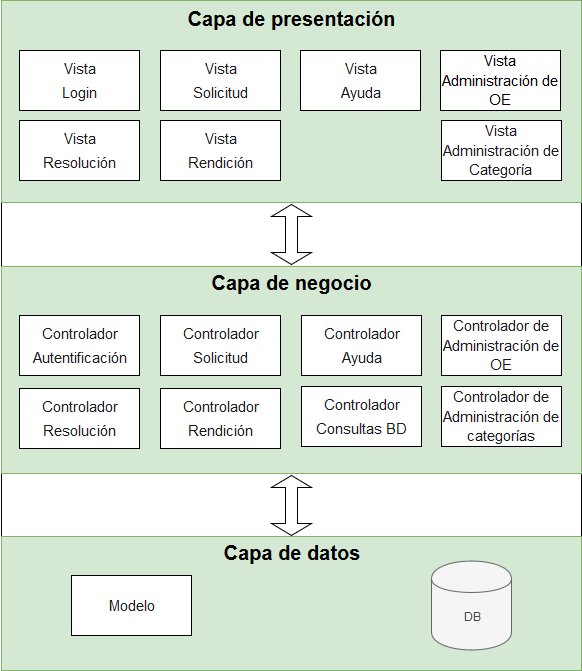
\includegraphics[width=0.8\textwidth]{Imagenes/Arquitectura_logica.png}
    \caption{\label{fig: Arquitectura_Logica}Arquitectura lógica del sistema.}
\end{figure}

Si bien se ha mencionado cómo es la arquitectura física que utiliza el sistema, en esta sección se habla acerca de la arquitectura lógica, la cual para efectos de esta memoria es \textbf{Modelo-Vista-Controlador (MVC)}. La elección de esta arquitectura se debe a que separa la interfaz de usuario de la lógica de negocio y el modelo de datos del sistema. Esto se realiza con el fin de evitar acoplamiento y facilitar los futuros mantenimientos dado que si se requiere de alguna modificación de una capa, las demás no se verán afectadas o en el caso de que se requiera el reemplazo completo de una capa, sólo se debe revisar las conexiones que tienen las demás capas a la que se está modificando para que funcione correctamente. Por ejemplo, cuando se requiere migrar la Base de datos, sólo se debe reemplazar los datos de conexión que se encuentran en la capa de Modelo y las otras capas no se verán afectadas. La \textbf{Figura \ref{sec:Arquitectura_Logica}} muestra la arquitectura lógica de la aplicación. A continuación se explica cada capa.

\begin{itemize}
    \item \textbf{Capa de Presentación: } Esta capa contempla todas las interfaces de usuario o vistas que posee el sistema. Cabe destacar que existen dos roles en el sistema, el de usuario común y el de administrador. Es por ello que la distribución de las vistas según el rol queda de la siguiente manera:
    \begin{enumerate*}[label=(\roman*)]
        \item Vista Solicitud,
        \item Vista Resolución y
        \item Vista Rendición 
      \end{enumerate*}
      son exclusivamente del usuario común mientras que 
      \begin{enumerate*}[label=(\roman*), start=4]
        \item Vista Administración OE y
        \item Vista Administración de Categoría
      \end{enumerate*}
      son exclusivos del rol del administrador del sistema. Por otra parte, existen vistas en que pueden interactuar ambos usuarios las cuales son: 
      \begin{enumerate*}[label=(\roman*), start=6]
        \item Vista Ayuda y
        \item Vista Login. 
      \end{enumerate*}
    \item \textbf{Capa de Negocio: }Esta capa contiene todos los controladores que la aplicación posee y es la capa intermediaria entre la Capa de Presentación y la Capa de Datos. A continuación, se procede a explicar cada uno de los controladores:
        \begin{itemize}
            \item Controlador Autentificación: Encargado de obtener y corroborar los datos de acceso de los distintos usuarios.
            \item Controlador Solicitud: Encargado de obtener y manipular los datos para confeccionar una solicitud que ingresa la OE interesada para enviarlos al Controlador Consultas BD y así sean registrados.
            \item Controlador Resolución: Encargado de obtener y manipular los datos de la Resolución enviada por la Institución que acredita la aceptación de la Solicitud realizada por la OE.
            \item Controlador Rendición: Encargado de obtener y manipular todos los datos que conlleva una Rendición, entre los cuales se considera los datos de las boletas y/o facturas y datos del encargado del evento. Todo esto con el fin de calcular el monto cercano o igual al solicitado por la OE para luego obtener el documento de rendición y a su vez enviar los datos al Controlador Consultas BD para que registre los datos ingresados.
            \item Controlador Ayuda: Encargado de obtener la información de manuales y preguntas frecuentes del sistema, entre otros, para enviarlos a la vista de ayuda que el usuario solicita. Este controlador no obtiene nada desde la vista de usuario, sólo obtiene la información que se encuentra en el servidor.
            \item Controlador de Administración de OE: Encargado de crear nuevas cuentas para las nuevas OE y modificar información de las ya existentes. 
            \item Controlador de Administración de Categorías: Encargado de gestionar nuevas categorías que serán utilizadas en la Solicitud y en la Rendición para mencionar en que fueron realizados los gastos.
            \item Controlador Consultas BD: Encargado de obtener los datos enviados desde los controladores para reenviarlos a la BD. Además, es el encargado de realizar otras consultas que son solicitadas por los controladores para obtener datos de la BD.
        \end{itemize}  
    \item \textbf{Capa de Datos: } Esta capa contempla el Modelo de Datos de la aplicación y las conexiones hacia la Base de datos.
\end{itemize}
